\section{光的吸收与辐射}

\begin{quotation}
``物理学,当今正处在一个新生的时代,上一个世纪还认为是正确的东西,
今天已暴露出了它的局限性……我们必须全力以赴去获得这些新知识……''\qquad 费米
\end{quotation}

原子光谱是由于光(电磁辐射)与原子相互作用产生的现象,在电磁辐射场中,原子可能吸收光的能量从低能级跃迁到高能级,或从高能级跃迁到低能级放出一定频率的光,这两种过程分别叫做光的吸收(Absorption)\index{Absorption: 吸收}和受激辐射(induced radiation)\index{Induced radiation: 受激辐射}。即使没有外加电磁辐射场,原子也可能自发地跃迁到较低能级上,并放出一定频率的光,称为自发辐射(spontaneous radiation)。

\begin{figure}[h]
\begin{center}
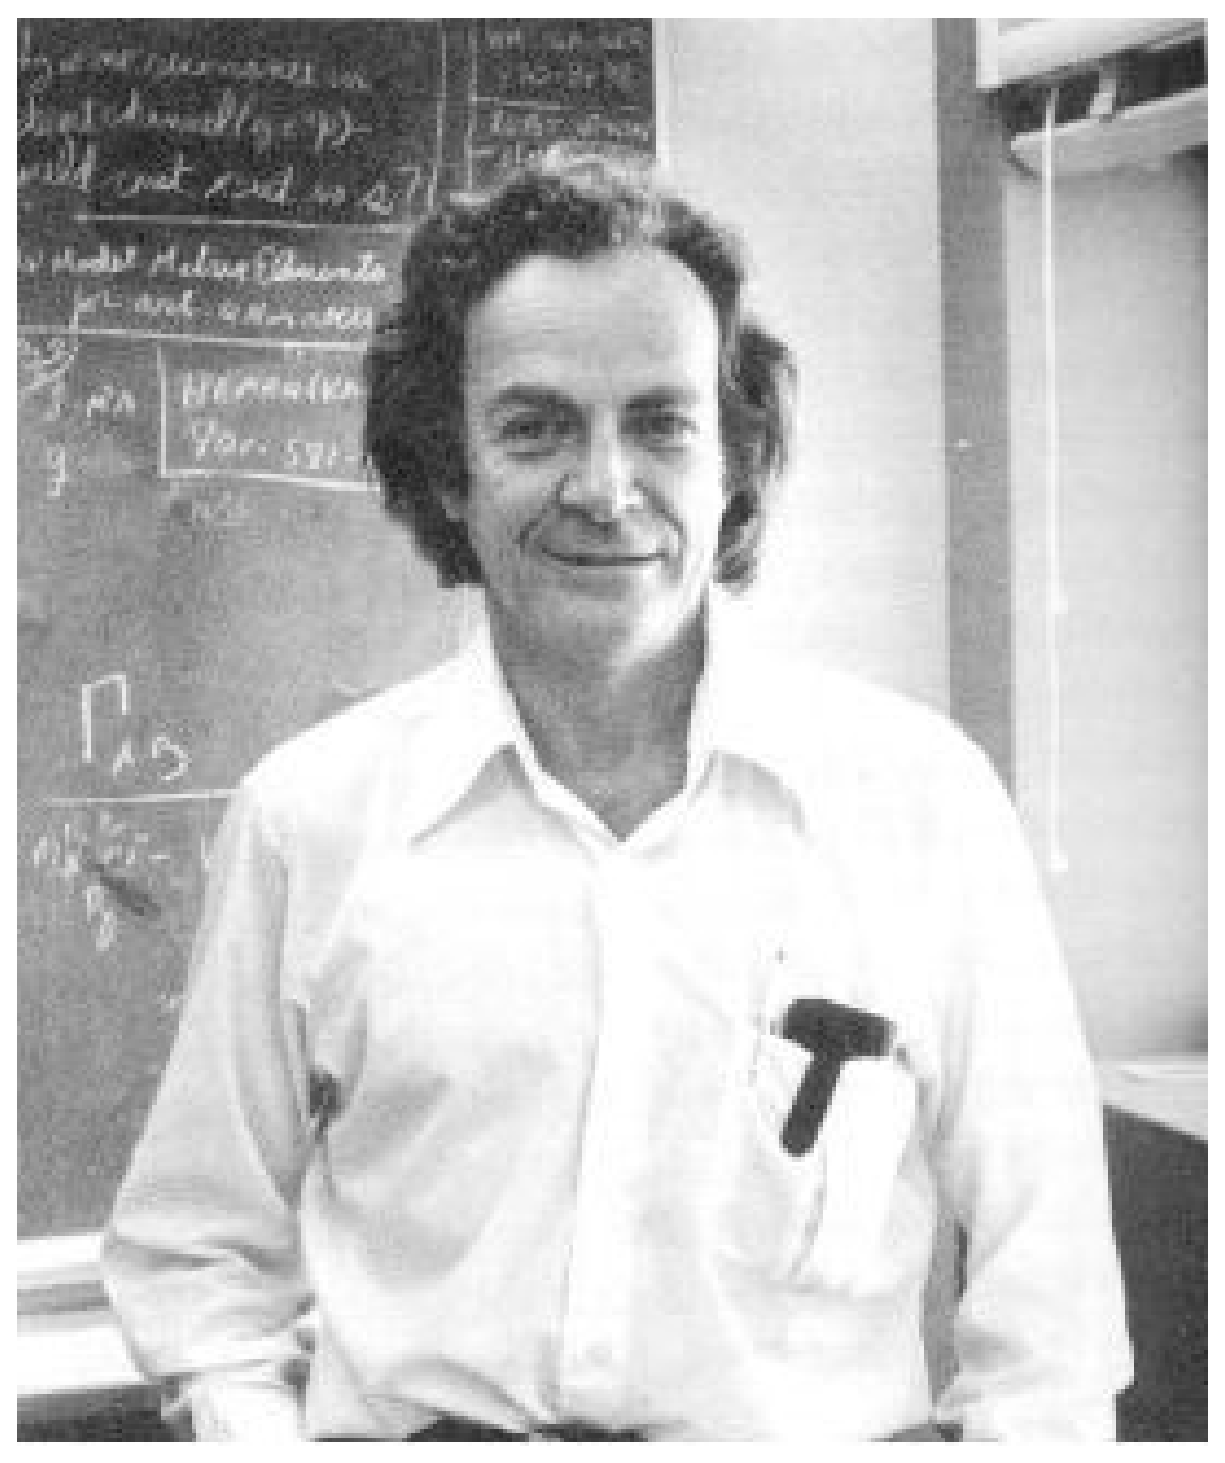
\includegraphics[clip,width=6cm]{Perturbation/feynman.ps}
\caption{费曼}
\end{center}
\end{figure}

原子光谱谱线的位置可由原子能级能量差解释$\nu  = \Delta E/h$,谱线相对强度则与能级间跃迁速率成正比。光的吸收与辐射的严格处理,
除应把原子系统视为量子力学系统外,我们还应将电磁辐射场进行量子化,
这样才能得到光子的产生或湮灭的物理图象,这需要用到量子电动力学(QED)的知识。量子电动力学是由费曼、施温格和朝永振一郎创立,它是目前最精确的物理理论\footnote{参考杨福家《原子物理学》第192页;

关于量子电动力学的通俗介绍,参考:费曼《QED:光和物质的奇异性》, 商务印书馆, 1996},并在从地球大小的100倍到原子核大小的百分之一尺度内经受着实验的考验。


我们还可以半经典地处理光的吸收与辐射,即把原子作为量子力学系统处理,而把电磁辐射场看作一个连续变化的经典电磁场(一个与时间有关的微扰),并使用含时微扰论计算原子跃迁速率。半经典理论可以直接计算光的吸收速率和受激辐射速率,但无法计算自发辐射速率(微扰消失,此时不适用微扰论)。但考虑到三种跃迁过程可以达到动态平衡,利用平衡条件我们可以求出自发辐射速率[Einstein 1917]。

\subsection{光的吸收与受激辐射}

假设入射光为平面单色光:

\begin{equation}\label{25-1}
\left\{ \begin{array}{l}
 {\rm E} = {\rm E}_0 \cos \left( {\omega t - k \cdot r} \right) \\
 {\rm B} = \sqrt {\varepsilon _0 \mu _0 } \frac{{k \times {\rm E}}}{{\left| k \right|}} = \frac{1}{c}\frac{{k \times {\rm E}}}{{\left| k \right|}} \\
 \end{array} \right.
\end{equation}

\subsubsection{偶极近似}

在原子尺度(用玻尔半径$a_0$表征)内,磁场对电子的影响要远小于电场对电子的影响:

\begin{equation}\label{25-2}
\frac{{\left| {ev \times {\rm B}} \right|}}{{\left| {e{\rm E}} \right|}} \sim \frac{v}{c} \sim \frac{{\alpha c}}{c} = \frac{1}{{137}}
\end{equation}

因此只需考虑电场的作用。在原子尺度内,
电场强度随空间的分布可以忽略,因此可看作是均匀电场:${\rm E} = {\rm
E}_0 \cos \omega
t$,在这种情况下讨论的跃迁称为偶极跃迁,这种近似称为偶极近似(Electric Dipole Approximation)\index{Electric Dipole Approximation: 电偶极近似}。

电子与外加电场相互作用:$H' =  - e\phi  = e{\rm E} \cdot {\vec r} =
e {\vec r} \cdot {\rm E}_0 \cos \omega t =  - {\vec D} \cdot {\rm
E}_0 \cos \omega t$


其中: $ - er$为电偶极矩\footnote{电偶极矩定义:$\vec D =
\sum\limits_i {q_i {\vec r_i} } $,电偶极矩\index{Electric dipole moment: 电偶极矩}在电场中的相互作用:$ -
\vec D \cdot \vec E$};



\subsubsection{跃迁速率}


\begin{equation}\label{25-3}
\begin{array}{l}
 a_{mk}^{(1)} (t) = \frac{1}{{i\hbar }}\int_0^t {dtH'_{mk} e^{i\omega _{mk} t} }  = \frac{{\left\langle m \right.\left| {e {\vec r} \cdot {\rm E}_0 } \right|\left. k \right\rangle }}{{2i\hbar }}\int_0^t {dt\left( {e^{i\omega t}  + e^{ - i\omega t} } \right)e^{i\omega _{mk} t} }  \\
  =  - \frac{{\left\langle m \right.\left| {e {\vec r} \cdot {\rm E}_0 } \right|\left. k \right\rangle }}{{2\hbar }}\left[ {\frac{{e^{i(\omega _{mk}  + \omega )t}  - 1}}{{\omega _{mk}  + \omega }} + \frac{{e^{i(\omega _{mk}  - \omega )t}  - 1}}{{\omega _{mk}  - \omega }}} \right] \\
 \end{array}
\end{equation}

由上式可见当$\omega  \sim  \pm \omega _{mk} $时, $a_{mk}^{(1)}
(t)$有显著的贡献, 否则随着偏离($\left| {\omega _{mk}  \pm \omega }
\right|$)的增大, $a_{mk}^{(1)} (t)$成反比变小, 而逐渐趋于零。


首先讨论原子吸收电磁辐射的跃迁, $E_m  > E_k $,当$\omega  \approx
\omega _{mk} $时, 引起$k \to m$的跃迁, 此时跃迁几率:

\begin{equation}\label{25-4}
 W_{k \to m} = \left| {a_{mk}^{(1)} (t)} \right|^2  = \frac{{| \left\langle m \right.\left| {e {\vec r} \cdot {\rm E}_0 } \right|\left. k \right\rangle |^2 }}{{4\hbar ^2 }}\frac{{\sin ^2 {\textstyle{{(\omega _{mk}  - \omega )t} \over 2}}}}{{[{\textstyle{{\omega _{mk}  - \omega } \over 2}}]^2 }}
\end{equation}

当时间$t$充分长后,上式可化为$\delta$函数的形式。

\begin{equation}\label{25-5}
\begin{array}{c}
W_{k \to m}  = \frac{{2\pi te^2 | \left\langle m \right.\left| {
{\vec r} \cdot {\rm E}_0 } \right|\left. k \right\rangle |^2
}}{{4\hbar ^2 }}\delta \left( {\omega _{mk}  - \omega } \right) \\
= \frac{{\pi te^2 | \left\langle m \right.\left| { {\vec r} \cdot {\rm
E}_0 } \right|\left. k \right\rangle |^2 }}{{2\hbar ^2 }}\delta
\left( {\omega _{mk}  - \omega } \right)\\
\end{array}
\end{equation}

跃迁速率:

\begin{equation}\label{25-6}
\begin{array}{c}
w_{k \to m}  = \frac{{\pi e^2 }}{{2\hbar ^2 }} | \left\langle m
\right|\left. { {\vec r} \cdot {\rm E}_0 \cos \theta } \right|\left.
k \right\rangle |^2 \delta \left( {\omega _{mk}  - \omega } \right) \\
= \frac{{\pi e^2 {\rm E}_0^2 }}{{2\hbar ^2 }}\left\langle {\cos ^2
\theta } \right\rangle | \left\langle m \right|\left. {\vec r}
\right|\left. k \right\rangle |^2 \delta \left( {\omega _{mk}  -
\omega } \right) \\
\end{array}
\end{equation}


其中$\theta$为电场方向与矢径方向夹角, $\left\langle {\cos ^2 \theta
} \right\rangle $是$\cos ^2 \theta
$对空间各角度的平均值。如入射光是非偏振光\footnote{根据曾谨言《量子力学·上册》pp567,需要计算矩阵元:$|W_{mk}|^2$,这里,$W=-\vec{D}\cdot
\vec{E}_0$,$\vec{D}=-e \vec{r}$,是电偶极矩。因此:$W=-\vec{D}
\cdot \vec{E}_0 = e \vec{r} \cdot \vec{E}_0$, 其中:$\vec{r} \cdot
\vec{E}_0 = x E_x^0 + y E_y^0 + z E_z^0 = r E_0 cos (\angle \vec{r},
\vec{E}_0)$, $\angle(\vec{r}, \vec{E}_0)$ 表示的是 $\vec{r}$ 与
$\vec{E}_0$ 之间的夹角。


$W_{mk} = \left<m|x E_x^0 + y E_y^0 + z E_z^0|k\right> =
\left<m|x|k\right>E_x^0 + \left<m|y|k\right>E_y^0 +
\left<m|z|k\right>E_z^0$,

即:$W_{mk} = \left<m|\vec{r}|k\right> \cdot \vec{E}_0 =
|\left<m|\vec{r}|k\right>| E_0 \cos \Theta$,这里 $\Theta$ 表示的是
${\left\langle {m} \right|\vec r\left| k \right\rangle }$ 与
$\vec{E}_0$ 之间的夹角。由于 ${\left\langle {m} \right|\vec r\left|
k \right\rangle }$ 矢量的方向是确定的,而自然光的 $\vec{E}_0$
则可取空间任意方向(参考: D. J. Griffiths, \textbf{Introduction to
Quantum Mechanics}, pp310)。因此 $\cos^2 \Theta$
对空间所有方向求平均的结果是 $1/3$ 。

现在,$\left| {W_{mk} } \right|^2  = \frac{{e^2 E_0^2 }}{3}\left|
{\left\langle {m} \right|\vec r\left| k \right\rangle } \right|^2
$。

},则:$\left\langle {\cos ^2 \theta } \right\rangle  = \frac{{\int
{d\Omega \cos ^2 \theta } }}{{\int {d\Omega } }} =
\frac{1}{3}$,$d\Omega  = \sin \theta d\theta d\varphi $。

跃迁速率:

\begin{equation}\label{25-7}
w_{k \to m}  = \frac{{\pi e^2 {\rm E}_0^2 }}{{6\hbar ^2 }} |
\left\langle m \right|\left. {\vec r} \right|\left. k \right\rangle
|^2 \delta \left( {\omega _{mk}  - \omega } \right)
\end{equation}

利用电磁辐射的能量密度公式,
振荡频率为$\omega$的电磁辐射所具有的能量密度:

\begin{equation}\label{25-8}
\rho (\omega ) = \overline {\left( {{\textstyle{{\varepsilon _0 } \over 2}}{\rm E}^2 (\omega ) + {\textstyle{1 \over {2\mu _0 }}}{\rm B}^2 (\omega )} \right)}  = 2\overline {\left( {{\textstyle{{\varepsilon _0 } \over 2}}{\rm E}^2 (\omega )} \right)}  = {\textstyle{1 \over 2}}\varepsilon _0 {\rm E}_0^2 (\omega )
\end{equation}

这里的平均是对时间求平均, 跃迁速率:

\begin{equation}\label{25-9}
\begin{array}{l}
w_{k \to m}  = \int {d\omega \frac{{\pi e^2 {\rm E}_0^2 (\omega
)}}{{6\hbar ^2 }} | \left\langle m \right|\left. {\vec r}
\right|\left. k \right\rangle |^2 \delta \left( {\omega _{mk}  -
\omega } \right)} \\
\qquad  = \frac{{\pi e^2 {\rm E}_0^2 (\omega _{mk}
)}}{{6\hbar ^2 }} | \left\langle m \right|\left. {\vec r}
\right|\left. k \right\rangle |^2 = \frac{{\pi e^2 \rho (\omega _{mk} )}}{{3\hbar ^2 \varepsilon _0 }}
| \left\langle m \right|\left. {\vec r} \right|\left. k
\right\rangle |^2 \\
\end{array}
\end{equation}

\subsubsection{选择定则}


矩阵元${\left\langle {m} \right|\vec r\left| k \right\rangle
}$可能有实部,也可能有虚部。即:$\left| {\left\langle {m}
\right|\vec r\left| k \right\rangle } \right|^2 = \text{Re}
\vec{r}_{mk}^2 + \text{Im} \vec{r}_{mk}^2$。

$\text{Re} \vec{r}_{mk}^2 = \text{Re} (x_{mk}^2 + y_{mk}^2 +
z_{mk}^2)$,  $\text{Im} \vec{r}_{mk}^2 = \text{Im} (x_{mk}^2 +
y_{mk}^2 + z_{mk}^2)$。

所以: $\left| {\left\langle {m} \right|\vec r\left| k \right\rangle
} \right|^2 = |\left<m|x|k\right>|^2 + |\left<m|y|k\right>|^2 +
|\left<m|z|k\right>|^2$, 即在 $|\left<m|\vec{r}|k\right>|^2$
中的取模运算兼有复数取模和向量取模两重含义。选择定则(selection
rules)将由对矩阵元$\left| {\left\langle {m} \right|\vec r\left| k
\right\rangle } \right|^2$ 的计算给出。

\index{Selection rules: 选择定则}

计算矩阵元:$| \left\langle m \right|\left. {\vec r} \right|\left. k
\right\rangle |^2  = | \left\langle m \right|\left. x \right|\left.
k \right\rangle |^2  + | \left\langle m \right|\left. y
\right|\left. k \right\rangle |^2  + | \left\langle m \right|\left.
z \right|\left. k \right\rangle |^2 $, 利用:

\begin{equation}\label{25-10}
\left\{ \begin{array}{l}
 x = r\sin \theta \cos \varphi  = \frac{r}{2}\sin \theta \left( {e^{i\varphi }  + e^{ - i\varphi } } \right) \\
 y = r\sin \theta \sin \varphi  = \frac{r}{{2i}}\sin \theta \left( {e^{i\varphi }  - e^{ - i\varphi } } \right) \\
 z = r\cos \theta  \\
 \end{array} \right.
\end{equation}

如果矩阵元$\left\langle m \right|\left. {\vec r} \right|\left. k
\right\rangle  =
0$,按照半经典理论偶极近似下,这种跃迁就不能实现,称为禁戒跃迁;$\left\langle
m \right|\left. {\vec r} \right|\left. k \right\rangle  \ne
0$的条件表示允许的跃迁,称为谱线的选择定则。


电子在中心力场中的状态可用波函数$\psi _{nlm}  = R_{nl} Y_{lm}
$表示,矩阵元为:$\left\langle m \right|\left. {\vec r}
\right|\left. k \right\rangle  \to \left\langle {n'l'm'}
\right.\left| {\vec r} \right|\left. {nlm} \right\rangle
$(右侧的$m$表示磁量子数)

利用递推关系:

\begin{equation}\label{25-11}
\left\{ \begin{array}{l}
 \cos \theta Y_{lm}  = \sqrt {\frac{{(l + 1)^2  - m^2 }}{{(2l + 1)(2l + 3)}}} Y_{l + 1,m}  + \sqrt {\frac{{l^2  - m^2 }}{{(2l - 1)(2l + 1)}}} Y_{l - 1,m}  \\
 e^{ \pm i\varphi } \sin \theta Y_{lm}  =  \mp \sqrt {\frac{{(l \pm m + 1)(l \pm m + 2)}}{{(2l + 1)(2l + 3)}}} Y_{l + 1,m \pm 1}  \pm \sqrt {\frac{{(l \mp m)(l \mp m - 1)}}{{(2l - 1)(2l + 1)}}} Y_{l - 1,m \pm 1}  \\
 \end{array} \right.
\end{equation}


积分可以化为径向部分和角度部分的乘积,由于径向部分积分不为0,只考虑角度部分积分就可得到跃迁定则。


由球谐函数的正交归一性,当$l' = l \pm 1$,$m' = m,m \pm
1$时,矩阵元$\left\langle {n'l'm'} \right.\left| {\vec r}
\right|\left. {nlm} \right\rangle  \ne 0$

因此偶极近似下,角量子数与磁量子数的选择定则:$\Delta l =  \pm 1$,$\Delta m = 0, \pm 1$


\subsection{自发辐射的爱因斯坦理论}

\begin{figure}[h]
\begin{center}
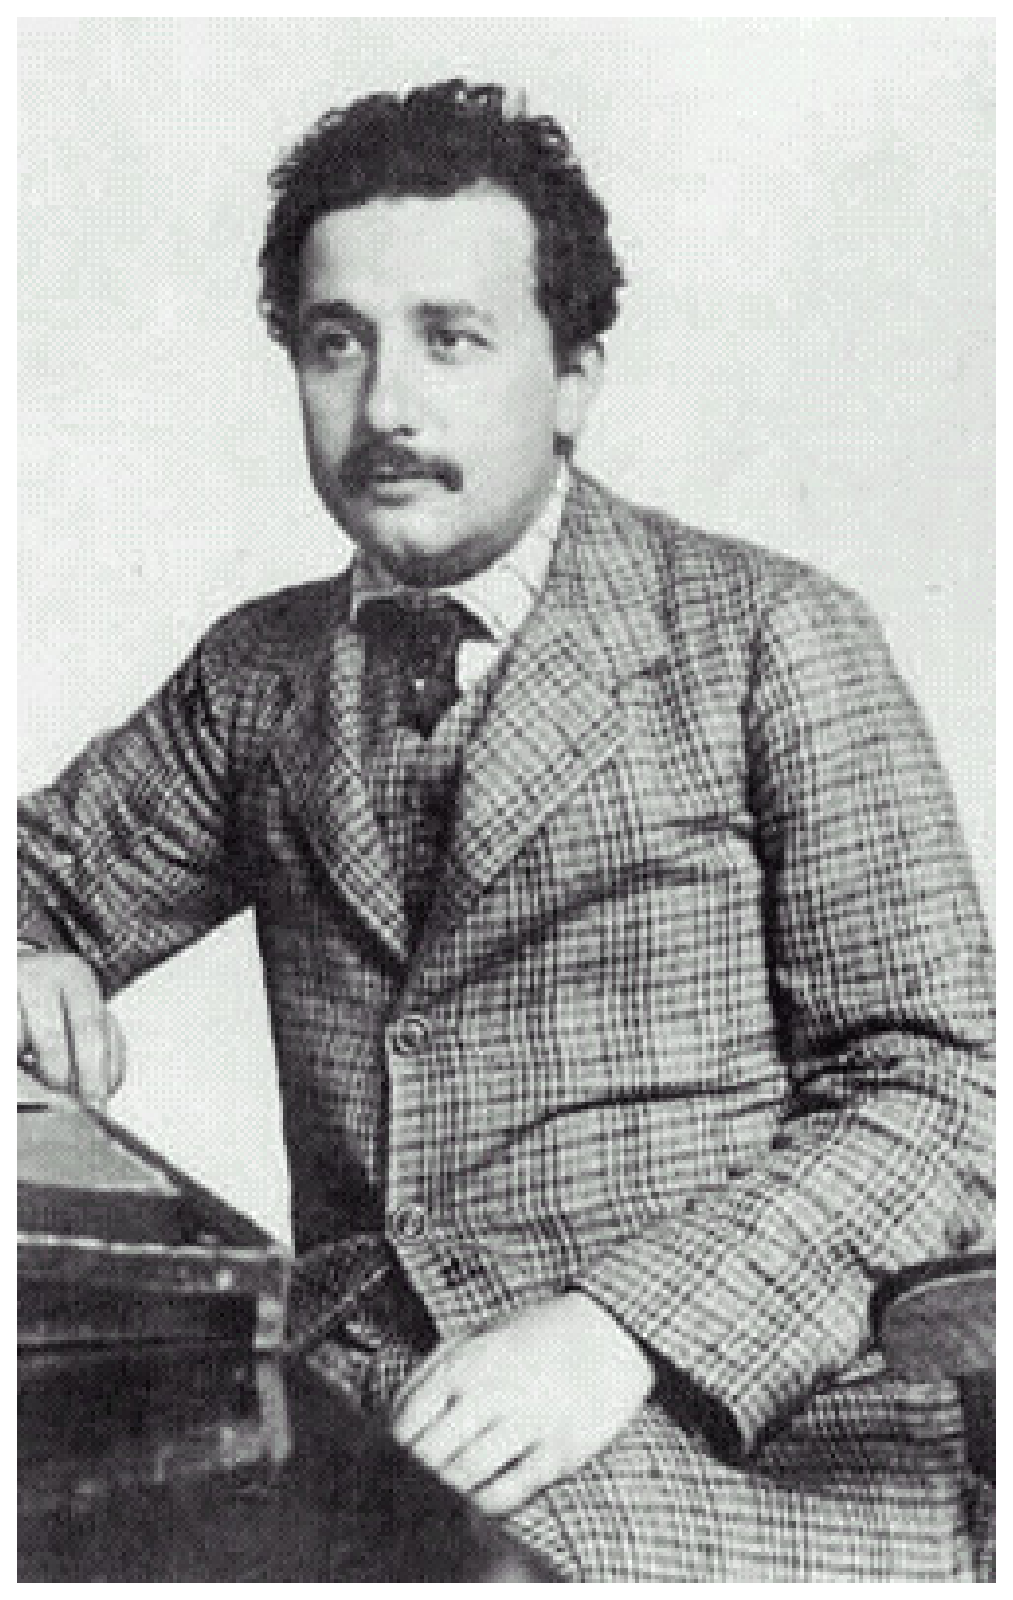
\includegraphics[clip,width=5cm]{Perturbation/einstein.ps}
\caption{爱因斯坦}
\end{center}
\end{figure}


原子吸收电磁辐射由$\left| k \right\rangle  \to \left| m \right\rangle $的速率为:

\begin{equation}\label{25-12}
w_{k \to m}  = \frac{{\pi e^2 | \left\langle m \right|\left. {\vec
r} \right|\left. k \right\rangle |^2 }}{{3\hbar ^2 \varepsilon _0
}}\rho (\omega _{mk} ) = B_{mk} \rho (\omega _{mk} )
\end{equation}

其逆过程,受激辐射原子由$\left| m \right\rangle  \to \left| k \right\rangle $的速率为:

\begin{equation}\label{25-13}
w_{m \to k}  = \frac{{\pi e^2 | \left\langle k \right|\left. {\vec
r} \right|\left. m \right\rangle |^2 }}{{3\hbar ^2 \varepsilon _0
}}\rho (\omega _{mk} ) = B_{km} \rho (\omega _{mk} )
\end{equation}

其中:吸收系数:

\begin{equation}\label{25-14}
B_{mk}  = \frac{{\pi e^2 | \left\langle m \right|\left. {\vec r}
\right|\left. k \right\rangle |^2 }}{{3\hbar ^2 \varepsilon _0 }}
\end{equation}

受激辐射系数:

\begin{equation}\label{25-15}
B_{km}  = \frac{{\pi e^2 | \left\langle k \right|\left. {\vec r}
\right|\left. m \right\rangle |^2 }}{{3\hbar ^2 \varepsilon _0 }}
\end{equation}

由于:$| \left\langle m \right|\left. {\vec r} \right|\left. k
\right\rangle | = | \left\langle k \right|\left. {\vec r}
\right|\left. m \right\rangle |$,所以:$B_{mk}  = B_{km} $;


假设电磁辐射场、$\left| k \right\rangle $,$\left| m \right\rangle $处于热平衡,温度为$T$;$n_k$表示占据$\left| k \right\rangle $的电子数,$n_m$表示占据$\left| m \right\rangle $的电子数;由于:$E_m  > E_k $,占据$\left| m \right\rangle $的电子有自发跃迁到较低状态$\left| k \right\rangle $的趋势,自发跃迁速率应正比于占据$\left| m \right\rangle $的电子数。

平衡条件:

\begin{equation}\label{25-16}
\frac{{dn_m }}{{dt}} = B_{mk} \rho (\omega _{mk} )n_k  - B_{km} \rho (\omega _{mk} )n_m  - A_{km} n_m  = 0
\end{equation}

其中$A_{km}$表示自发辐射系数。

$B_{mk} \rho (\omega _{mk} )n_k  = B_{km} \rho (\omega _{mk} )n_m  + A_{km} n_m $, $ \Rightarrow $


$\rho (\omega _{mk} ) = \frac{{A_{km} n_m }}{{B_{mk} n_k  - B_{km} n_m }} = \frac{{A_{km} }}{{B_{mk} \frac{{n_k }}{{n_m }} - B_{km} }}$


利用玻尔兹曼关系:$n_m  \propto e^{ - E_m /k_B T} $, $\frac{{n_k }}{{n_m }} = e^{(E_m  - E_k )/k_B T}  = e^{\hbar \omega _{mk} /k_B T} $

\begin{equation}\label{25-17}
\rho (\omega _{mk} ) = \frac{{A_{km} }}{{B_{mk} \frac{{n_k }}{{n_m }} - B_{km} }} = \frac{{A_{km} }}{{B_{km} }}\frac{1}{{e^{\hbar \omega _{mk} /k_B T}  - 1}}
\end{equation}

根据普朗克公式: $u_T (\nu )d\nu  = \frac{{8\pi h\nu ^3 }}{{c^3 }}
\cdot \frac{1}{{e^{\frac{{h\nu }}{{k_B T}}}  - 1}}d\nu $, 即:$\rho
(\omega )d\omega  = \frac{{\hbar \omega ^3 }}{{\pi ^2 c^3 }} \cdot
\frac{1}{{e^{\frac{{\hbar \omega }}{{k_B T}}}  - 1}}d\omega $

得到:

\begin{equation}\label{25-18}
A_{km}  = \frac{{\hbar \omega ^3 }}{{\pi ^2 c^3 }}B_{km}  =
\frac{{\hbar \omega ^3 }}{{\pi ^2 c^3 }} \cdot \frac{{\pi e^2 |
\left\langle k \right|\left. {\vec r} \right|\left. m \right\rangle
|^2 }}{{3\hbar ^2 \varepsilon _0 }} = \frac{{\omega ^3 e^2 }}{{3\pi
\varepsilon _0 \hbar c^3 }} | \left\langle k \right|\left. {\vec r}
\right|\left. m \right\rangle |^2
\end{equation}

所以自发辐射\index{Spontaneous emission: 自发辐射}的选择定则与受激辐射和吸收的选择定则相同。


\subsection{真空涨落}

量子力学认为,真空态并不是一个``一无所有''的状态,
它仍然有能量的涨落,即电磁辐射场的涨落,这种真空态的涨落``激发''了自发辐射。

\index{Vacuum fluctuation: 真空涨落}

根据受激辐射跃迁速率公式:

\begin{equation}\label{25-19}
w_{m \to k}  = \frac{{\pi e^2 | \left\langle k \right|\left. {\vec
r} \right|\left. m \right\rangle |^2 }}{{3\hbar ^2 \varepsilon _0
}}\rho (\omega _{mk} )
\end{equation}

我们需要计算真空态对应的能量密度$\rho (\omega _{mk} ) = g(\omega )dE$

根据态密度公式[第2节 黑体辐射]:$g(\nu ) = \frac{1}{V}\frac{{dN(\nu )}}{{d\nu }} = \frac{1}{{L^3 }}\frac{{8\pi \nu ^2 L^3 }}{{c^3 }} = \frac{{8\pi \nu ^2 }}{{c^3 }}$

变量变换后,态密度:$g(\omega ) = \frac{{\omega ^2 }}{{\pi ^2 c^3 }}$

电磁辐射场可看作是一系列不同频率的振子,量子化后,能量最小单元为$\hbar \omega $(光子),产生或湮灭一个光子需要$\hbar \omega $的能量[第19节 线性谐振子与占有数表象]。所以:$dE = \hbar \omega $

能量密度:$\rho (\omega _{mk} ) = g(\omega )dE = \frac{{\hbar \omega _{mk} ^3 }}{{\pi ^2 c^3 }}$

得到:$w_{m \to k}  = \frac{{\pi e^2 | \left\langle k \right|\left.
{\vec r} \right|\left. m \right\rangle |^2 }}{{3\hbar ^2 \varepsilon
_0 }}\frac{{\hbar \omega ^3 }}{{\pi ^2 c^3 }} = \frac{{\omega ^3 e^2
}}{{3\pi \varepsilon _0 \hbar c^3 }} | \left\langle k \right|\left.
{\vec r} \right|\left. m \right\rangle |^2
$,与使用热平衡条件求得的结果(\ref{25-18})相同。



\subsection{磁偶极跃迁}

如果我们只考虑磁场的作用,并取微扰哈密顿:

\begin{equation}\label{25-20}
H' =  - \mu  \cdot {\rm B}_0 \cos \omega t
\end{equation}

得到磁偶极近似。

$\mu _L  =  - g_L \frac{e}{{2m}}L$, $\mu _s  =  - g_s \frac{e}{{2m}}s$; $g_L  = 1$, $g_s  = 2$

所以:$\mu  = \mu _L  + \mu _s  =  - \frac{e}{{2m}}\left( {L + 2s} \right)$,

微扰哈密顿为:

\begin{equation}\label{25-21}
H' = \frac{e}{{2m}}{\rm B}_0  \cdot \left( {L + 2s} \right)\cos \omega t
\end{equation}

矩阵元:$\left\langle b \right|\left. {H'} \right|\left. a \right\rangle  = \frac{e}{{2m}}\left\langle b \right|\left. {{\rm B}_0  \cdot \left( {L + 2s} \right)} \right|\left. a \right\rangle \cos \omega t$

\begin{eqnarray*}
c_{ba}^{(1)} (t) & = & \frac{1}{{i\hbar }}\int_0^t {dtH'_{ba} e^{i\omega _{ba} t} } \\
{} & = &  \frac{1}{{i\hbar }}\frac{e}{{4m}}\int_0^t {dt\left\langle b \right|\left. {{\rm B}_0  \cdot \left( {L + 2s} \right)} \right|\left. a \right\rangle \left[ {e^{i(\omega _{ba}  + \omega )t}  + e^{i(\omega _{ba}  - \omega )t} } \right]}  \\
{} & = &  - \frac{{e{\rm B}_0  \cdot \left\langle b \right|\left. {\left( {L + 2s} \right)} \right|\left. a \right\rangle }}{{4\hbar m}}\left[ {\frac{{e^{i(\omega _{ba}  + \omega )t}  - 1}}{{\omega _{ba}  + \omega }} + \frac{{e^{i(\omega _{ba}  - \omega )t}  - 1}}{{\omega _{ba}  - \omega }}} \right] 
\end{eqnarray*}

跃迁几率:

\begin{equation}\label{25-22}
W_{a \to b}  = \left| {c_{ba}^{(1)} (t)} \right|^2  = \frac{{e^2 |
\left\langle b \right|{\rm B}_0  \cdot \left. {\left( {L + 2s}
\right)} \right|\left. a \right\rangle |^2 }}{{16\hbar ^2 m^2
}}\frac{{\sin ^2 {\textstyle{{(\omega _{ba}  - \omega )t} \over
2}}}}{{[{\textstyle{{\omega _{ba}  - \omega } \over 2}}]^2 }}
\end{equation}


$t$趋于无穷时,可化为$\delta$函数形式:

\begin{equation}\label{25-23}
\begin{array}{c}
W_{a \to b}  = \frac{{e^2 | \left\langle b \right|{\rm B}_0  \cdot
\left. {\left( {L + 2s} \right)} \right|\left. a \right\rangle |^2
}}{{16\hbar ^2 m^2 }}2\pi t\delta \left( {\omega _{ba}  - \omega }
\right) \\
\qquad = \frac{{e^2 \pi t | \left\langle b \right|{\rm B}_0  \cdot
\left. {\left( {L + 2s} \right)} \right|\left. a \right\rangle |^2
}}{{8\hbar ^2 m^2 }}\delta \left( {\omega _{ba}  - \omega } \right)\\
\end{array}
\end{equation}

跃迁速率:

\begin{equation}\label{25-24}
\begin{array}{c}
w_{a \to b}  = \frac{{e^2 \pi | \left\langle b \right|{\rm B}_0
\cdot \left. {\left( {L + 2s} \right)} \right|\left. a \right\rangle
|^2 }}{{8\hbar ^2 m^2 }}\delta \left( {\omega _{ba}  - \omega }
\right) \\
= \frac{{e^2 {\rm B}_0^2 \pi \left\langle {\cos ^2 \theta }
\right\rangle | \left\langle b \right|\left. {\left( {L + 2s}
\right)} \right|\left. a \right\rangle |^2 }}{{8\hbar ^2 m^2
}}\delta \left( {\omega _{ba}  - \omega } \right)
\end{array}
\end{equation}

假设磁场振动方向在空间各方向都有:$\left\langle {\cos ^2 \theta } \right\rangle  = \frac{1}{3}$

\begin{eqnarray*}
w_{a \to b} &  = & \int {d\omega \frac{{e^2 {\rm B}_0^2 (\omega )\pi
}}{{24\hbar ^2 m^2 }} | \left\langle b \right|\left. {\left( {L +
2s} \right)} \right|\left. a \right\rangle |^2 \delta \left( {\omega
_{ba}  - \omega } \right)}  \\
{} & = & \frac{{e^2 {\rm B}_0^2 (\omega _{ba}
)\pi }}{{24\hbar ^2 m^2 }} | \left\langle b \right|\left. {\left( {L
+ 2s} \right)} \right|\left. a \right\rangle |^2
\end{eqnarray*}

能量密度:

$\rho (\omega ) = \overline {\left( {{\textstyle{{\varepsilon _0 } \over 2}}{\rm E}^2 (\omega ) + {\textstyle{1 \over {2\mu _0 }}}{\rm B}^2 (\omega )} \right)}  = 2\overline {\left( {{\textstyle{1 \over {2\mu _0 }}}{\rm B}^2 (\omega )} \right)}  = {\textstyle{1 \over {2\mu _0 }}}{\rm B}_0^2 (\omega )$

利用:${\rm B}_0^2 (\omega ) = 2\mu _0 \rho (\omega )$, 得到:

\begin{equation}\label{25-25}
w_{a \to b}  = \frac{{\pi \mu _0 e^2 \rho (\omega _{ba} )}}{{12\hbar
^2 m^2 }} | \left\langle b \right|\left. {\left( {L + 2s} \right)}
\right|\left. a \right\rangle |^2
\end{equation}

磁偶极跃迁速率与电偶极跃迁速率之比\footnote{利用:$\left\langle \mu  \right\rangle ^2  \sim \left( {\frac{e}{{2m}}} \right)^2 \hbar ^2 $, $\left\langle D \right\rangle ^2  \sim e^2 a_0^2 $, $a_0  = \frac{\hbar }{{mc\alpha }}$}为:

\begin{equation}\label{25-26}
\begin{array}{c}
\frac{{w_{a \to b} }}{{w_{k \to m} }} \sim \frac{{\pi \varepsilon _0 \mu _0 \rho (\omega )\left\langle \mu  \right\rangle ^2 }}{{\pi \rho (\omega )\left\langle D \right\rangle ^2 }} = \frac{{\left( {{\textstyle{e \over {2m}}}} \right)^2 \hbar ^2 }}{{c^2 e^2 a_0^2 }} \\
\sim \left( {\frac{\hbar }{c}} \right)^2 \left( {\frac{1}{{ma_0 }}} \right)^2  = \left( {\frac{\hbar }{{mca_0 }}} \right)^2  = \alpha ^2 \\
\end{array}
\end{equation}

可见磁偶极跃迁要比电偶极跃迁慢$\alpha ^2 $倍,或说:磁偶极跃迁导致的驰豫时间比电偶极跃迁驰豫时间长$\left( {137} \right)^2  \approx 1 \times 10^4 $倍\footnote{$\frac{{dn_m }}{{dt}} =  - A_{km} n_m $, $n_m (t) = n_m (0)e^{ - A_{km} t}  = n_m (0)e^{ - t/\tau } $, 因此: $\tau  \sim \frac{1}{{A_{km} }}$}。

\subsection{自旋翻转速率}

含自旋波函数一般写为:


\begin{equation}\label{25-27}
\psi (r,s_z ,t) = \left( {\begin{array}{*{20}c}
   {\psi _1 (r,t)}  \\
   {\psi _2 (r,t)}  \\
\end{array}} \right) = \psi _1 (r,t)\chi _ +   + \psi _1 (r,t)\chi _ -
\end{equation}

磁相互作用会导致自旋翻转,在磁偶极近似下,设初态为:$\psi _k \chi _ +  $,末态为:$\psi _{k'} \chi _ -  $

\index{Spin-flip: 自旋翻转}

矩阵元:

$\begin{array}{l}
 \left\langle {\psi _{k'} \chi _ -  } \right.\left| {L + 2s} \right.\left| {\psi _k \chi _ +  } \right\rangle  = \left\langle {\psi _{k'} \chi _ -  } \right.\left| L \right.\left| {\psi _k \chi _ +  } \right\rangle  + 2\left\langle {\psi _{k'} \chi _ -  } \right.\left| s \right.\left| {\psi _k \chi _ +  } \right\rangle  \\
  = \left\langle {\psi _{k'} } \right|L\left| {\psi _k } \right\rangle \left\langle {{\chi _ -  }}
 \mathrel{\left | {\vphantom {{\chi _ -  } {\chi _ +  }}}
 \right. \kern-\nulldelimiterspace}
 {{\chi _ +  }} \right\rangle  + 2\left\langle {{\psi _{k'} }}
 \mathrel{\left | {\vphantom {{\psi _{k'} } {\psi _k }}}
 \right. \kern-\nulldelimiterspace}
 {{\psi _k }} \right\rangle \left\langle {\chi _ -  } \right|s\left| {\chi _ +  } \right\rangle \\
 = 0 + 2\delta _{k'k} \left\langle {\chi _ -  } \right|s\left| {\chi _ +  } \right\rangle  \\
 \end{array}$

$k = k'$时:

$\begin{array}{l}
 \left\langle {\psi _{k'} \chi _ -  } \right.\left| {L + 2s} \right.\left| {\psi _k \chi _ +  } \right\rangle ^2  = 4\left\langle {\chi _ -  } \right|s\left| {\chi _ +  } \right\rangle ^2  \\
 = 4\left[ {\left\langle {\chi _ -  } \right|s_x \left| {\chi _ +  } \right\rangle ^2  + \left\langle {\chi _ -  } \right|s_y \left| {\chi _ +  } \right\rangle ^2  + \left\langle {\chi _ -  } \right|s_z \left| {\chi _ +  } \right\rangle ^2 } \right] \\
  = 4\left[ {\left\langle {\chi _ -  } \right|s_x \left| {\chi _ +  } \right\rangle ^2  + \left\langle {\chi _ -  } \right|s_y \left| {\chi _ +  } \right\rangle ^2  + 0} \right] \\
 \end{array}$

$\left\langle {\chi _ -  } \right|s_x \left| {\chi _ +  } \right\rangle  = \frac{\hbar }{2}\left( {\begin{array}{*{20}c}
   0 & 1  \\
\end{array}} \right)\left( {\begin{array}{*{20}c}
   0 & 1  \\
   1 & 0  \\
\end{array}} \right)\left( {\begin{array}{*{20}c}
   1  \\
   0  \\
\end{array}} \right) = \frac{\hbar }{2}$
,


$\left\langle {\chi _ -  } \right|s_y \left| {\chi _ +  } \right\rangle  = \frac{\hbar }{2}\left( {\begin{array}{*{20}c}
   0 & 1  \\
\end{array}} \right)\left( {\begin{array}{*{20}c}
   0 & { - i}  \\
   i & 0  \\
\end{array}} \right)\left( {\begin{array}{*{20}c}
   1  \\
   0  \\
\end{array}} \right) = \frac{\hbar }{2}i$

所以:

$\left\langle {\psi _{k'} \chi _ -  } \right.\left| {L + 2s} \right.\left| {\psi _k \chi _ +  } \right\rangle ^2  = 4\left[ {\left\langle {\chi _ -  } \right|s_x \left| {\chi _ +  } \right\rangle ^2  + \left\langle {\chi _ -  } \right|s_y \left| {\chi _ +  } \right\rangle ^2 } \right] = 2\hbar ^2 $


跃迁速率:

\begin{equation}\label{25-28}
w_{ \uparrow  \downarrow }  = \frac{{\pi \mu _0 \rho (\omega _{ \downarrow  \uparrow } )e^2 }}{{6m^2 }}
\end{equation}

在金属中传导电子自旋翻转速率比电子动量改变速率慢$\alpha ^2 $倍,或说电子自旋翻转驰豫时间比电子动量驰豫时间长$\left( {137} \right)^2  \approx 1 \times 10^4 $倍,$\tau _m  \gg \tau _e $。即电子自旋可以较长时间地保持其自旋取向,有利于我们实现以控制电子自旋状态为机制的电子学器件,即自旋电子学器件。


\subsection*{阅读与思考}

\begin{itemize}

\item 阅读文献,写篇关于``自旋电子学''的读书报告。

``量子微芯片还有多远'', 《科学美国人》中文版, 第30-37页, 第9期, 2002

冯端主编《材料科学导论》, 化学工业出版社, 第303-310页, 2002

\end{itemize}
